\ffigbox[\FBwidth]{%
\caption{\centering Instance initiale pour le \textsc{Vertex Cover}}\label{fig:dm1_ex01_f3}
}{
    \fbox{
        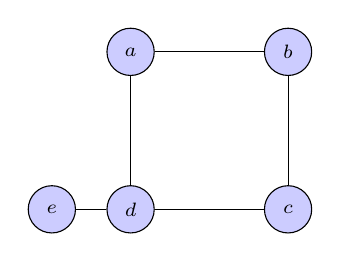
\begin{tikzpicture}[scale=1, main node/.style={circle, draw, fill=blue!20, inner sep=1pt, font=\scriptsize, minimum size=6mm, text=black}]
            % les sommets initiaux
            \node[main node] (a) at (0,0) {\(a\)};
            \node[main node] (b) at (2, 0) {\(b\)};
            \node[main node] (c) at (2,-2) {\(c\)};
            \node[main node] (d) at (0,-2) {\(d\)};
            \node[main node] (e) at (-1,-2) {\(e\)};

            % les arcs avec capacités
            \draw (a) edge (b);
            \draw (b) edge (c);
            \draw (c) edge (d);
            \draw (d) edge (a);
            \draw (d) edge (e);
            
        \end{tikzpicture}
    }
}